\section{Current Electricity}




\subsection{Kirchhoff's circuit laws}

Kirchhoff's laws\index{Kirchhoff's laws} are two rules that deal with the current and voltage in a circuit

they were first formulated by German physicist \emph{Gustav Robert Kirchhoff} in 1845

the two rules allow for analysis of complex circuits in the field of electrical engineering

\subsection{First law}

\begin{ilight}
	\keypoint{Kirchhoff's first law}\index{Kirchhoff's laws!first law}, also called \keypoint{Kirchhoff's current law} (KCL), states that for any point in a circuit, sum of currents flowing in equals sum of currents going out: \begin{empheq}[box=\tcbhighmath]{equation*}{\sum I_\text{in} = \sum I_\text{out}}\end{empheq}
\end{ilight}

Recall currents are produced by movement of electric charges so Kirchhoff's first law is therefore a consequence of \emph{conservation of electric charge}. 

\begin{marginfigure}
	\vspace{-21pt}
	\begin{center}
		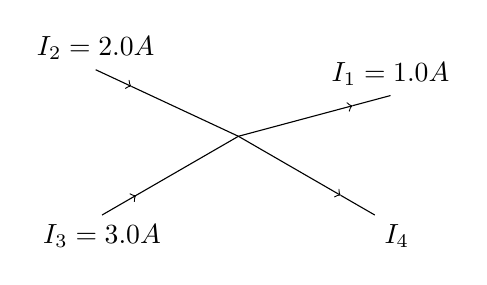
\begin{tikzpicture}
		\draw[->] (0:0) -- (15:1.5) ;
		\draw (15:1.5) -- (15:2) node[above]{$I_1 = 1.0 \text{ A}$};
		\draw[->] (155:2) node[above]{$I_2 = 2.0 \text{ A}$} -- (155:1.5) ;
		\draw (155:1.5) -- (0:0);
		\draw[->] (210:2) node[below] {$I_3= 3.0 \text{ A}$} -- (210:1.5)  ;
		\draw (210:1.5) -- (0:0);
		\draw[->] (0:0) -- (330:1.5) ;
		\draw (330:1.5) -- (330:2) node[below right]{$I_4$};
		\end{tikzpicture}
	\end{center}
	\vspace{-20pt}
\end{marginfigure}

\example{The diagram shows part of an electric circuit. The values of $I_1$, $I_2$ and $I_3$ are labelled. Calculate the current $I_4$.}

\begin{soln} applying the first law: $I_2 + I_3 = I_1 + I_4$
	
	\eqskip $\RA I_4 = 2.0 + 3.0 - 1.0 = 4.0$ A \end{soln}
	


\subsection{Second law}

\begin{ilight}
	\keypoint{Kirchhoff's second law}\index{Kirchhoff's laws!second law}, also known as \keypoint{Kirchhoff's voltage law} (KVL), states that for any closed loop in a circuit, sum of all e.m.f.'s of supplies is equal to sum of potential differences across resistors: \begin{empheq}[box=\tcbhighmath]{equation*}{\sum \mathcal{E} = \sum V }\end{empheq}
\end{ilight}

Recall e.m.f. and p.d. are both defined as energy transfer per unit charge. The e.m.f. of a supply is electrical energy produced per unit charge. The p.d. across a resistor gives electrical energy consumed per unit charge.
So Kirchhoff's second law is a consequence of \emph{energy conservation}.

Signs for $\mathcal{E}$ and $V$ depend on the choice of loop orientation.

% \begin{figure}[ht]
% 	\centering
% 	\begin{minipage}{0.24\textwidth}
% 		\centering
% 		\begin{circuitikz}
% 		\draw (2,0) to[battery1, l_=$\mathcal{E}$] (0,0);
% 		\draw[<-] (2,-1.5) [out=150, in=30] to (0,-1.5);
% 		\node at (1,-0.9) {loop};
% 		\end{circuitikz}
% 	\caption{$+\mathcal{E}$}
% 	\end{minipage}\hfil
% 	\begin{minipage}{0.24\textwidth}
% 		\centering
% 		\begin{circuitikz}
% 			\draw (2,0) to[battery1, l_=$\mathcal{E}$] (0,0);
% 			\draw[->] (2,-1.5) [out=150, in=30] to (0,-1.5);
% 			\node at (1,-0.9) {loop};
% 		\end{circuitikz}
% 		\caption{$-\mathcal{E}$}
% 	\end{minipage}\hfil
% 	\begin{minipage}{0.24\textwidth}
% 		\centering
% 		\begin{circuitikz}[european resistors]
% 			\draw (0,0) to[R, l^=$R$] (3,0);
% 			\draw[->] (2.5,0) -- (2.6,0) node[above] {$I$};
% 			\draw[<-] (2.5,-1.5) [out=150, in=30] to (0.5,-1.5);
% 			\node at (1.5,-0.9) {loop};
% 		\end{circuitikz}
% 		\caption{$V = +IR$}
% 	\end{minipage}\hfil
% 	\begin{minipage}{0.24\textwidth}
% 		\centering
% 		\begin{circuitikz}
% 			\draw (0,0) to[R, l^=$R$] (3,0);
% 			\draw[->] (2.5,0) -- (2.6,0) node[above] {$I$};
% 			\draw[->] (2.5,-1.5) [out=150, in=30] to (0.5,-1.5);
% 			\node at (1.5,-0.9) {loop};
% 		\end{circuitikz}
% 		\caption{$V = -IR$}
% 	\end{minipage}
% \end{figure}



% \begin{figure}[ht]
% 	\vspace*{-24pt}
% 	\centering
% 	\begin{circuitikz}[european resistors,scale=0.75]
% 		\draw (0,3) to [battery,l=$\mathcal{E}_1$] (4,3) to [R=$R_2$] (4,0);
% 		\draw (0,0) to [R=$R_1$] (0,3);
% 		\draw (0,0)  to [battery1] (4,0);
% 		\draw[Green, thick, dashed, ->] (3.0, 1.8597) arc(21.79:338.21:1.2 and 0.9);
% 		\node at (2,-0.9) {$\mathcal{E}_2$};
% 	\end{circuitikz}
% 	\vspace*{-10pt}
% \end{figure}

\example{For the circuit shown, find an expression, in terms of $\mathcal{E}$ and $R$, for the electric current flowing through the resistors.}

\begin{soln} apply KVL for the closed loop shown:


	\centering
	
	$ \mathcal{E}_1 - \mathcal{E}_2 = IR_1 + IR_2 $
	
	\eqyskip $ I = \frac{\mathcal{E}_1 - \mathcal{E}_2}{R_1 + R_2} $
	
	\end{soln}
	


\begin{marginfigure}
	\vspace*{-21pt}
	\centering
	\begin{circuitikz}[european resistors,scale=0.8]
		\draw (0,4) to [battery,l=$\mathcal{E}_1$] (3,4) to [R=$R_1$] (6,4) node[right]{B};
		\draw (0,2) node[left]{F} to [battery1,l=$\mathcal{E}_2$] (3,2) to [R=$R_2$] (6,2) node[right]{C};
		\draw (0,4) node[left]{A} -- (0,0) node[left]{E} to [R=$R_3$] (6,0) node[right]{D}-- (6,4);
		\draw[blue,->] (3.1,4) -- (2.9,4) node[midway, above]{$I_1$};
		\draw[blue,->] (3.1,2) -- (2.9,2) node[midway, above]{$I_2$};
		\draw[blue,->] (1.1,0) -- (1.3,0) node[midway, above]{$I_3$};
	\end{circuitikz}
	\vspace*{-16pt}
\end{marginfigure}

\example{The diagram shows a circuit where e.m.f. of the batteries and the values of resistance are all known. Write down the equations for the currents $I_1$, $I_2$ and $I_3$ using Kirchhoff's laws.}\footnote[][2cm]{The solutions are: $I_1 = \frac{(R_2+R_3)\mathcal{E}_1 - R_3 \mathcal{E}_2}{(R_1 + R_3)(R_2+R_3) - R_3^2}$, $I_2 = \frac{(R_2+R_3)\mathcal{E}_2 - R_3 \mathcal{E}_1}{(R_1 + R_3)(R_2+R_3) - R_3^2}$, $I_3 = \frac{R_1 \mathcal{E}_2 + R_2 \mathcal{E}_1}{(R_1 + R_3)(R_2+R_3) - R_3^2}$}

\begin{soln} apply KCL for point $C$ or $F$: $ I_1 + I_2 = I_3 \quad  $ \hspace*{21pt} \ding{172}

apply KVL for loop $AEDBA$: $\mathcal{E}_1 = I_1 R_1 + I_3 R_3$  \hspace*{7.5pt} \ding{173}

apply KVL for loop $FEDCF$: $\mathcal{E}_2 = I_2 R_2 + I_3 R_3$ \hspace*{5pt} \ding{174}

in principle, $I_1$, $I_2$ and $I_3$ can be solved from the three equations


one can also apply KVL for loop $AFCBA$ to write: $\mathcal{E}_1 - \mathcal{E}_2 = I_1 R_1 - I_2 R_2$

this equation looks complex but is simply \ding{173}$-$\ding{174}, which is not an independent equation

when writing down equations using KVL, choosing simpler loops gives easier equations \end{soln}


\subsection{Resistor networks}

For a network of resistors, it is useful to treat the combination as a single resistor. We can derive formula for series and parallel resistors using Kirchhoff's laws.

\subsection{Series resistors}

\begin{figure}[ht]
	\centering
	\begin{circuitikz}[european resistors]
	\draw (0,0) -- (1,0) to[R,l^=$R_1$] (4,0) to[R,l^=$R_2$] (6,0) to[R,l^=$R_3$] (9,0) -- (10,0);
	\draw[->] (1,0) -- (1.2,0) node[above]{$I$};
	\foreach \x/\xlabel in {1.5/1,4/2,6.5/3} \draw[<->] (\x,-1) --++ (2,0) node[midway, above]{$V_\xlabel$};
	\end{circuitikz}
	\caption{three resistors in series}
\end{figure}

Take three series resistors as shown. The current through each resistor is the same: $I = I_1 = I_2 = I_3$. The e.m.f. however must be split as p.d. across the three resistors: $V_\text{total} = V_1 + V_2 + V_3$

Dividing both sides by $I$, we have: $\frac{V_\text{total}}{I} = \frac{V_1}{I} + \frac{V_2}{I} + \frac{V_3}{I}$

So combined resistance for the three resistors is: $R_\text{total} = R_1 + R_2 + R_3$

In general, if there are $n$ resistors in series, then: \begin{empheq}[box=\tcbhighmath]{equation*}{R_\text{total} = R_1 + R_2 + \cdots + R_n} \end{empheq}

If one of the resistors in a series network increases, then $R_\text{total}$ would increase. Adding an additional resistor to a network in series, would cause $R_\text{total}$ to increase.



\subsection{parallel resistors}

\begin{marginfigure}
	\vspace*{-35pt}
	\centering
	\begin{circuitikz}[european resistors,scale=0.9]
		\foreach \y/\ylabel in {1.5/1, 0/2, -1.5/3} {
			\draw (-1.5,\y) --++ (0.5,0) to[R, l^=$R_\ylabel$] (1.5,\y);
			\draw[->] (-0.9,\y) --++ (0.1,0) node[above]{$I_\ylabel$};
		}
		\draw (-1.5, -1.5) --++ (0,3) (1.5, -1.5) --++ (0,3);
		\draw (-3, 0) --++ (1.5,0) (1.5,0) --++ (1.5,0);
		\draw[->] (-2.4,0) --++ (0.1,0) node[above]{$I$};
		\draw[<->] (-1.2,-2.4) -- (1.2,-2.4) node[midway, above]{$V$};
	\end{circuitikz}
	\caption{three resistors in parallel}
	\vspace*{-16pt}
\end{marginfigure}

let's next take three parallel resistors

same p.d. across each resistor: $V = V_1 = V_2 = V_3$

current is shared: $I_\text{total} = I_1 + I_2 + I_3$

divide both sides by $V$: $\frac{I_\text{total}}{V} = \frac{I_1}{V} + \frac{I_2}{V} + \frac{I_3}{V}$

so combined resistance has: $\frac{1}{R_\text{total}} = \frac{1}{R_1} + \frac{1}{R_2} + \frac{1}{R_3}$

in general, for $n$ resistors in parallel:

{
	\centering
	
	\begin{empheq}[box=\tcbhighmath]{equation*}{\frac{1}{R_\text{total}} = \frac{1}{R_1} + \frac{1}{R_2} + \cdots + \frac{1}{R_n} } \end{empheq}
	
}


\cmt if one of the resistors in a parallel network increases, then $R_\text{total}$ would increase

\cmt adding an additional resistor to a network in parallel, then $R_\text{total}$ would decrease

\cmt if $n$ identical resistors $R_0$ are connected in parallel, then $R_\text{total}  = \frac{1}{n}R_0$


\begin{marginfigure}
	\vspace*{-20pt}
	\centering
	\begin{circuitikz}[european resistors,scale=0.8]
		\draw (3,1) to [R,l_=$R_1$] (0,1) -- (0,4) to [battery,l=$\mathcal{E}$] (7,4) -- (7,1) -- (6.5,1);
		\draw (3,0) -- (3,2) to [R=$R_2$] (6.5,2) -- (6.5,0);
		\draw (3,0) to [R=$R_3$] (6.5,0);
	\end{circuitikz}
	\vspace*{-16pt}
\end{marginfigure}

\example{In the circuit shown, the battery has an e.m.f. $\mathcal{E}=18$ V, and the resistors have $R_1=6.0$ $\Omega$, $R_2=4.0$ $\Omega$ and $R_3=12$ $\Omega$. (a) Find the total resistance of all external resistors. (b) Find the current through the battery. (c) Find the p.d. across $R_1$, $R_2$ and $R_3$. (d) Find the total power dissipated in $R_2$ and $R_3$.}

\begin{soln} total resistance: $R = R_1 + \left( \frac{1}{R_2} + \frac{1}{R_2} \right)^{-1} = 6.0 + \left( \frac{1}{4.0} + \frac{1}{12} \right)^{-1} = 6.0 + 3.0 = 9.0 \text{ } \Omega$

\eqyskip current through battery: $I = \frac{\mathcal{E}}{R} = \frac{18}{9.0} = 2.0 \text{ A}$

p.d across $R_1$: $ V_1 = I R_1 = 2.0 \times 6.0 = 12 \text{ V}$

p.d across $R_2$ and $R_3$: $V_2 = V_3 = \mathcal{E} - V_1 = 18 - 12 = 6.0 \text{ V}$

power dissipated in $R_2$: $P_2 = \frac{V_2^2}{R_2} = \frac{6.0^2}{4.0} = 9.0 \text{ W}$

power dissipated in $R_3$: $P_3 = \frac{V_3^2}{R_3} = \frac{6.0^2}{12} = 3.0 \text{ W}$ \end{soln}

\subsection{practical circuits}

\subsection{power supplies \& internal resistance}

all real power sources have \emph{internal resistance}\index{internal resistance}

examples are resistance in electrolytic solution of a battery or in coils for a generator

\begin{marginfigure}
	\vspace{-12pt}
	\centering
	\begin{circuitikz}[european resistors, xscale=0.8, yscale=0.95]
		\draw (0,0) -- (0,3) -- (1,3) to[battery,l^=$\mathcal{E}$] (3,3) to[R,l^=$r$] (5,3) -- (6,3) -- (6,0) to[R,l_=$R$] (0,0);
		\draw[dashed] (1,1.8) rectangle (5,4.2);
		\draw[->] (0,1.6) -- (0,1.5) node[left]{$I$};
	\end{circuitikz}
	\vspace{-20pt}
\end{marginfigure}

a practical battery can be thought as the combination of an ideal battery with e.m.f. $\mathcal{E}$ and internal resistance $r$

if this battery is connected to a circuit of external resistance $R$, applying the Kirchhoff's laws, we write:

{
	\centering
	
	\begin{empheq}[box=\tcbhighmath]{equation*}{\mathcal{E} = V_R + V_r = I(R+r)}\end{empheq}
	
}

$V_R$ is called the \keypoint{terminal p.d.} across the battery

$V_r$ is called the \keypoint{lost volts} in the internal resistance

\cmt \keypoint{internal resistance} of a battery can be defined as ratio of lost volts to current in battery

\cmt when a current flows through a battery, terminal p.d. will be less than battery's e.m.f.

this is because some voltage is lost due to internal resistance


\cmt current in the circuit is given by: $I = \frac{\mathcal{E}}{R+r}$

\begin{compactitem}
	\item[--] maximum current when terminals are shorted-out, i.e., when external load $R=0$
	
	greatest current is therefore: $I_\tmax = \frac{\mathcal{E}}{r}$
	
	though this current is limited to some finite value, this still causes great heating effects
	
	this should be avoided because battery may be destroyed if temperature gets too high
	
	\item[--] battery drives no current for an open circuit, i.e., $I \to 0$ if external resistance $R \to \infty$
	
	in this case, there is no lost volts, so terminal p.d. equals e.m.f.
\end{compactitem}

\cmt note that there are several different notions of electrical powers

\begin{compactitem}
	\item[--] total power generated in battery is: $P_\text{total} = I\mathcal{E} = I^2 (R+r)$

	\item[--] power delivered to external circuit is: $P_R = I V_r = I^2 R$

	\item[--] power dissipated (rate of thermal energy produced) in battery is: $P_r = I V_r = I^2 r$
\end{compactitem}

\example{A car battery has an e.m.f. of 20 V and an internal resistance of 0.50 $\Omega$. When a starter motor of resistance of 3.50 $\Omega$ is connected to the battery, find (a) the current supplied to the motor, (b) the p.d. across the battery terminals, (c) the power at which the motor operates.}

\begin{soln} current in circuit: $I = \frac{\mathcal{E}}{R+r} = \frac{20}{3.50 + 0.50} = 5.0 \text{ A} $

terminal p.d.: $V_R = IR = 5.0 \times 3.50 = 17.5 \text{ V}$

power of motor: $P_R = IV_R = 5.0 \times 17.5 = 87.5 \text{ W} \, \text{  or }\, P_R = I^2 R = 5.0^2 \times 3.50 = 87.5 \text{ W}$ \end{soln}

\example{A battery of e.m.f. $12$ V is connected to a network of total resistance of 22 $\Omega$. The current through the battery is $0.50$ A. Find (a) the internal resistance of the battery, (b) the total power produced by battery, (c) the power dissipated in battery.}

\begin{soln} lost volts: $V_r = \mathcal{E} - IR = 12 - 0.50 \times 22 = 1.0 \text{ V}$

internal resistance: $r = \frac{V_r}{I} = \frac{1.0}{0.50} = 2.0 \text{ }\Omega$

power produced by battery: $P_\text{total} = I\mathcal{E} = 0.50 \times 12 = 6.0 \text{ W}$

power dissipated in battery: $P_r = I V_r = 0.50 \times 1.0 = 0.50 \text{ W} \, \text{  or }\, P_r = I^2 r = 0.50^2 \times 2.0 = 0.50 \text{ W}$ \end{soln}

\example{An electric heater is operating at a working p.d. of 200 V. A current of 5.0 A is driven by a voltage source of 230 V. The source has an internal resistance of 4.0 $\Omega$ and the resistance of the connecting wires is not negligible. Find (a) the lost volts in the source, (b) the resistance of the wires, (c) the useful power from the source, (d) the efficiency of this circuit.}

\begin{soln} lost volts: $V_r = I r = 5.0 \times 4.0 = 20 \text{ V}$

p.d. across wires: $V_\text{wire} = \mathcal{E} - V_\text{heater} - V_r = 230 - 200 - 20 = 10 \text{ V}$

resistance of wires: $ R_\text{wire} = \frac{V_\text{wire}}{I} = \frac{10}{5.0} = 2.0 \text{ }\Omega$

useful power: $P_\text{useful} = P_\text{heater} = I V_\text{heater} = 5.0 \times 200  = 1000 \text{ W}$

efficiency: $\eta = \frac{P_\text{useful}}{P_\text{total}} = \frac{I V_\text{heater}}{I\mathcal{E}} = \frac{200}{230} \approx 87\%$ \end{soln}


\example{A cell of e.m.f. $\mathcal{E}$ and internal resistance $r$ is connected in series with a variable resistor $R$. $R$ is gradually increased from zero. (a) Suggest how the p.d. across the battery terminals change when $R$ is increased. (b) For larger values of $R$, power delivered to $R$ decreases. Suggest the advantage, despite the low power output, of using this cell in a circuit of larger resistance.}

\begin{soln} as $R$ increases, current in circuit decreases

less voltage is lost in cell, so terminal p.d. will increase

for same reason, less power is lost in cell, so higher efficiency for the circuit

more explicitly, terminal p.d. $V_R = I R = \frac{\mathcal{E}R}{R+r}$, and efficiency $ \eta = \frac{P_R}{P_\text{total}} = \frac{I^2 R}{I^2(R+r)} = \frac{R}{R+r}$

from these we can tell: if $R\up$, then $\frac{R}{R+r} \up$, so $V_R \up$ and $ \eta \up$ \end{soln}




\subsection*{power output from a practical battery}

power output to external components is
\begin{equation*}
P_\text{out} = I^2R = \left( \frac{\mathcal{E}}{R+r} \right)^2 R
\end{equation*}

assuming $\mathcal{E}$ and $r$ are constant, then $P_\text{out}$ only depends on the external load $R$ of the circuit

the diagram below show how $P_\text{out}$ varies with $R$

\begin{figure}[htp]
	\centering
	\begin{tikzpicture}[scale = 0.95]
	\draw [thick, <->] (9,0) node[below]{$R$} -- (0,0) --(0,5) node[left]{$P_\text{out}$};
	\draw [thick,blue,domain=0:8.4,samples=30,smooth,variable=\x] plot (\x, {16*\x/(\x+1)^2});
	\draw [dashed] (0,4) node[left]{$P_\tmax=\frac{\mathcal{E}^2}{4r}$} -- (1,4) -- (1,0) node[below]{$r$};
	\draw [->] (2,4.4) node[above right,note]{maximum power output when $R=r$} -- (1.2,4.1);
	\draw [->] (7,3.0) node[note]{$P_\text{out}$ decreases as current\\ decreases with load $R$} -- (7,2.0);
	\draw [->] (4.5,0.8) node[note]{low $P_\text{out}$ for small external load $R$ \\ as large fraction of e.m.f. is lost on $r$} -- (0.3,0.8);
	\end{tikzpicture}
	\caption{variation of output power $P_\text{out}$ from a power supply to an external resistor $R$}
\end{figure}

\cmt when $R$ is small, only a small fraction of e.m.f. is output as terminal p.d.

so most of the power generated is lost on the internal resistance of the source

\cmt as $R$ gradually increases, terminal p.d. increases, causing a temporary rise in $P_\text{out}$

however, increase in terminal p.d. is compensated by a reduction in electric current

\cmt when $R$ continues to increase, current becomes so small that $P_\text{out}$ gradually tends to zero

\cmt maximum power output is archived when $R=r$, this power is given by: $P_\text{out,max} = \frac{\mathcal{E}^2}{4r}$ 
\footnote{For any two positive numbers $x$ and $y$, $x+y \geq 2\sqrt{xy}$ where the equality holds if and only if $x=y$. We then have $P_\text{out} = \frac{\mathcal{E}^2 R}{(R+r)^2} = \frac{\mathcal{E}^2}{R + \frac{r^2}{R} + 2r} \leq \frac{\mathcal{E}^2}{2\sqrt{R \cdot \frac{r^2}{R}} + 2r} = \frac{\mathcal{E}^2}{4r}$. To obtain the greatest power, the condition $R=\frac{r^2}{R}$, i.e., $R=r$ must be satisfied.}




\subsection*{measurement of e.m.f. and internal resistance of a power supply}

\begin{marginfigure}
	\vspace{-30pt}
	\begin{center}
		\begin{circuitikz}[european resistors, xscale=0.8,yscale=0.75]
			\draw (0,0) -- (0,3) to[battery,l^=$\mathcal{E} \quad r$] (5,3) to[rmeter, t=A] (5,0) to[vR] (0,0);
			\draw (0.8,0) -- (0.8,-1.6) to[rmeter, t=V] (4.2,-1.6) -- (4.2,0);
			\node at (2.5, 0.7) {$R$};
		\end{circuitikz}
	\end{center}
	\vspace{-20pt}
\end{marginfigure}

the circuit for determining e.m.f. and internal resistance of an unknown power source is shown on the right

terminal p.d. $V_R$ is measured by the voltmeter

current $I$ in circuit is measured by the ammeter

one can vary $R$ to obtain a set of measurements for $I$ and $V$

values of $V$ can then be plotted against values of $I$


since $V_R=\mathcal{E} - Ir$, data points should fall in a straight line

\begin{compactitem}
	\item[--] $\mathcal{E}$ is $y$-intercept of the graph
	
	\item[--] $r$ is given by the negative gradient
\end{compactitem}



\begin{figure}[ht]
	\centering
	\begin{tikzpicture}[xscale = 1.35, yscale=1.5]
	\draw [thick, <->] (8,0) node[below]{$I$} -- (0,0) --(0,3.6) node[left]{$V$};
	\draw [thick,blue] (0,3) node[left]{\textcolor{black}{$\mathcal{E}$}} -- (7,0) node[below]{\textcolor{black}{$I_\tmax$}};
	\draw [->] (6.5,1.5) node[note]{maximum current $I_\tmax = \frac{\mathcal{E}}{r}$\\when terminals are shorted-out} -- (6.8,0.3);
	\draw [->] (1.6,1) node[note]{$V=\mathcal{E} - Ir$ \\$\text{gradient} = -r$\\$y\text{-intercept}=\mathcal{E}$} -- (2.8,1.6);
	\draw [->] (3.5,3.0) node[note]{terminal p.d. tends to e.m.f. when \\connected to a high-resistance component} -- (0.4,3.0);
	\end{tikzpicture}
	\caption{variation of terminal p.d across a battery against the current flowing through it}
\end{figure}



\subsection{practical ammeters \& voltmeters}

when connected into a circuit, ideal ammeters/voltmeters do not affect original currents

so ideal ammeter has zero resistance, and ideal voltmeter has infinite resistance

but in practice, ammeters have non-zero resistance, voltmeter have finite resistance

to find current through an ammeter/p.d. a voltmeter, treat them as normal resistor

reading on ammeter/voltmeter gives the current through/p.d. across itself

\begin{marginfigure}
	\vspace*{-18pt}
	\centering
	\begin{tikzpicture}[xscale=1.25, yscale=1.1]
	\draw(3.6,3) to[battery,l_=$\mathcal{E}$] (0,3) -- (0,0) to[rmeter, t=V] (3.6,0) -- (3.6,1.5) to[rmeter, t=A] (3.6,3);
	\draw (0,1.5) to[R,l^=$R$] (3.6,1.5);
	\end{tikzpicture}
	\vspace*{-18pt}
\end{marginfigure}

\example{The diagram shows a simple circuit. The battery has a negligible internal resistance and an e.m.f. of 8.0 V. The resistor has a fixed resistance of 20 $\Omega$. (a) Find the readings shown on the ammeter and the voltmeter if both meters are ideal. (b) Instead, the ammeter has a non-zero resistance of 1.0 $\Omega$ and the voltmeter has a resistance of 60 $\Omega$, what are the true readings displayed on the two meters?}

\begin{soln} if both meters are ideal, then $I = \frac{\mathcal{E}}{R} = \frac{8.0}{20} = 0.40 \text{ A}$, and $V = \mathcal{E} = 8.0 \text{ V}$

for non-ideal case, total resistance in circuit: $R_\text{total} = R_A + \left( \frac{1}{R} + \frac{1}{R_V} \right)^{-1} = 1.0 + \left( \frac{1}{20} + \frac{1}{60} \right)^{-1} = 16 \text{ }\Omega$

current through ammeter: $I = \frac{\mathcal{E}}{R_\text{total}} = \frac{8.0}{16} = 0.50 \text{ A}$

p.d. across voltmeter: $V = \mathcal{E} - V_A = \mathcal{E} - I R_A = 8.0 - 0.50 \times 1.0 = 7.5 \text{ V} $ \end{soln}


\subsection{potential dividers}

one type of useful circuit is the potential divider\index{potential divider}

a \keypoint{potential divider} can produce an output voltage that is a fraction of input voltage

\begin{marginfigure}
	\vspace*{-5pt}
	\centering
	\begin{circuitikz}[european resistors,scale=0.9]
	\draw (0,5) to[battery,l^=$\mathcal{E}$] (0,0) -- (2,0) to[R,l_=$R_2$] (2,2.5) to[R,l_=$R_1$] (2,5) -- (0,5);
	\draw[<->] (3,0.02) --++ (0,2.46) node[right, midway]{$V_2$};
	\draw[<->] (3,2.52) --++ (0,2.46) node[right, midway]{$V_1$};
	\foreach \y in {0, 2.5, 5} \draw (2.9, \y) --++ (0.2,0);
	\end{circuitikz}
	\vspace*{-21pt}
\end{marginfigure}

a typical potential divider circuit is shown

p.d. across $R_1$ and $R_2$ satisfy the relationship:

{
	\centering
	
	$ \frac{V_1}{V_2} = \frac{IR_1}{IR_2} \RA \frac{V_1}{V_2} = \frac{R_1}{R_2}$
	
}

we also have the relation: $V_1 + V_2 = \mathcal{E}$

these together give the \emph{potential divider equation}:

{
	\centering
	
	\begin{empheq}[box=\tcbhighmath]{equation*}{V_1 = \frac{R_1}{R_1+R_2}\times\mathcal{E}} \end{empheq} \begin{empheq}[box=\tcbhighmath]{equation*}{V_2 = \frac{R_2}{R_1+R_2}\times\mathcal{E}} \end{empheq}
	
}

this means $R_1$ and $R_2$ divide up the p.d. supplied to them

proportion of p.d. share depends on relative resistance values


\begin{marginfigure}
	\vspace*{8pt}
	\centering
	\begin{circuitikz}[european resistors,scale=0.9]
		\draw (0,2) -- (0,0) -- (2,0) to[vR] (2,2.5) to[R] (2,5) -- (0,5) -- (0,3);
		\draw (2,2.5) -- (4,2.5) to[rmeter, t=V] (4,0) -- (2,0);
		\node[right] at (2.25,3.75) {$R_0=10\text{ }\Omega$};
		\node[right] at (2.25,1.25) {$R$};
		\draw (0,2.08) circle (0.08);
		\draw (0,2.92) circle (0.08);
		\node at (0,2.5) {15 V};
	\end{circuitikz}
	\vspace*{-25pt}
\end{marginfigure}


\example{The diagram shows an electric circuit incorporating a power supply of negligible internal resistance and a high-resistance voltmeter. Determine the range of voltage reading on the voltmeter as the variable resistor $R$ is adjusted over its full range from 0 $\Omega$ to 50 $\Omega$.}

\begin{soln} $V_\tmin = \frac{R_\tmin}{R_\tmin + R_0} \times V_\text{in} = \frac{0}{0+10}\times 15 \RA V_\tmin = 0 \text{ V}$

\eqyskip $V_\tmax = \frac{R_\tmax}{R_\tmax + R_0} \times V_\text{in} = \frac{50}{50+10}\times 15 \RA V_\tmax = 12.5 \text{ V}$

so voltage reading ranges from 0 to 12.5 V \end{soln}


\subsection*{bridge circuits}



\emph{bridge circuits} can be designed by altering the potential divider circuit
\footnote{The bridge circuit we will be looking at is known as the \emph{Wheatstone bridge}. The circuit design was invented by British scientist \emph{Samuel Hunter Christie} in 1833 and later improved by another British scientist \emph{Charles Wheatstone} in 1843.}

by balancing two legs of a bridge circuit, an unknown resistance can be measured

\begin{figure}[ht]
	\vspace*{-5pt}
 \begin{flushright}
     
 
	\begin{circuitikz}[european resistors,scale=0.9]
		\draw (6,0) -- (6,3.75) to[battery] (0,3.75) -- (0,0); 
		\draw (0,2) to[R] (3,2) to[R] (6,2);
		\draw (0,0) to[R] (3,0) to[vR] (6,0);
		\draw (3,0) to[rmeter, t=G] (3,2);
		\node[above] at (1.5, 2.25) {$R_1$};
		\node[above] at (4.5, 2.25) {$R_2$};
		\node[above] at (1.5, 0.25) {$R_x$};
		\node[above] at (4.5, 0.25) {$R_v$};
		\node[above] at (3,4.25) {$\mathcal{E}$};
	\end{circuitikz}
 \end{flushright}
  \forceversofloat
	\vspace*{-5pt}
 
\end{figure}

the circuit diagram shows a typical bridge circuit

$R_x$ is the unknown resistance to be measured

resistance of $R_1$, $R_2$ and variable resistor $R$ are known 

$R$ is adjusted until no current flows through galvanometer, the bridge is then said to be \emph{balanced}

p.d. share between $R_1$ and $R_2$ is same as p.d. share between $R_x$ and $R$: $ \frac{R_1}{R_2} = \frac{R_x}{R}$


so resistance of $R_x$ can be determined to great accuracy
\footnote{Measurement with the Wheatstone bridge circuit can be extremely accurate because the scheme illustrates the concept of a difference measurement, which can be done to very high accuracy.}



\begin{marginfigure}
	\vspace*{5pt}
	\centering
	\begin{circuitikz}[european resistors,scale=0.9]
		\draw (6,0) -- (6,4) to[battery] (0,4) -- (0,0); 
		\draw (0,2) to[R] (3,2) to[R] (6,2);
		\draw (0,0) to[R] (3,0) to[vR] (6,0);
		\draw (3,0) to[rmeter, t=V] (3,2);
		\node[above] at (1.5, 2.25) {$R_1 = 10 \text{ }\Omega$};
		\node[above] at (4.5, 2.25) {$R_2 = 20 \text{ }\Omega$};
		\node[above] at (1.5, 0.25) {$R_3 = 25 \text{ }\Omega$};
		\node[above] at (4.5, 0.25) {$R_4$};
		\node[above] at (3,4.5) {$\mathcal{E}=24 \text{ V}$};
	\end{circuitikz}
	\vspace*{-16pt}
\end{marginfigure}



\example{Four resistors are connected to a battery as shown. (a) If the variable resistor $R_4$ is adjusted to have a resistance of 35 $\Omega$, what is the reading on the voltmeter? (b) If the voltmeter reads zero, what is the resistance for $R_4$?}

\begin{soln}
    
 (a) p.d. across $R_1$: $V_1 = \frac{10}{20+10}\times24 = 8.0 \text{ V}$

\eqyskip\hspace*{1.2em} p.d. across $R_3$: $V_3 = \frac{25}{35+25}\times24 = 10.0 \text{ V}$

\eqyskip\hspace*{1.2em} voltmeter reading: $V = V_3 - V_1 = 10.0 -8.0 = 2.0 \text{ V}$

(b) $V=0$ means p.d. share between $R_1$ and $R_2$ is same as p.d. share between $R_3$ and $R_4$
\begin{equation*}
	\frac{R_1}{R_2} = \frac{R_3}{R_4} \RA \frac{10}{20} = \frac{25}{R_4} \RA R_4 = 50 \text{ }\Omega 
\end{equation*}
\end{soln}

\subsection*{potentiometer}

another useful type of potential divider is the \emph{potentiometer}\index{potentiometer}

p.d.'s or e.m.f.'s can be compared in terms of length quantities with a potentiometer

\begin{figure}[ht]
	\centering
	\vspace*{-5pt}
	\begin{circuitikz}[yscale=0.8]
		\draw (0,0) node[left]{$A$} -- (0,3) node[left]{$X$} to [battery,l=$\mathcal{E}_d$] (8,3) node[right]{$Y$} -- (8,0) node[right]{$B$};
		\foreach \x in {0,1,...,7} \draw[ultra thick, gray] (\x,0) --++ (0.25,0.03) --++ (0.5,-0.06) --++ (0.25,0.03);
		\draw (0,0) -- (0,-3) node[left]{$Z$} to [battery1, l=$\mathcal{E}_t$] (5,-3) node[right]{$W$} to [rmeter, t=G] (5,0) node[above]{$P$};
		\draw[-{Latex[length=5mm, width=1.5mm]}] (5,-0.3) --++ (0,0.3);
		\draw (5.2,-0.4) --++ (1.2,-0.8) node[right,twoline]{sliding\\contact};
		\draw (7,0.15) --++ (1.8, 1) node[right,twoline]{resistance\\wire};
		\draw (4.4,3.2) --++ (0.7, 0.6) node[right]{driver cell};
		\draw (2.7,-3.2) --++ (0.7, -0.6) node[right]{test cell};
	\end{circuitikz}
	\vspace*{-5pt}
\end{figure}

the diagram shows a potentiometer being used to measure the e.m.f. of a unknown cell

suppose driver cell has no internal resistance and an e.m.f. of $\mathcal{E}_d$ that is already known

to find e.m.f. of test cell, we adjust position of contact $P$ until galvanometer shows zero

taking loop $XAPBYX$, we have: $\mathcal{E}_d = V_{AB} = I R_{AB}$

taking loop $ZAPWZ$, we have: $\mathcal{E}_t = V_{r,t} + V_{AP} = \cancelto{0}{ir_t} + I R_{AP} = I R_{AP}$

compare the two equations, we find: $\frac{\mathcal{E}_t}{\mathcal{E}_d} = \frac{R_{AP}}{R_{AB}}$

recall resistance of uniform wire is proportional to its length: $\frac{R_{AP}}{R_{AB}} = \frac{AP}{AB}$

now ratio of e.m.f.'s of the two cells are related to ratio of two lengths $AP$ and $AB$

e.m.f. of test cell is given by: $ \mathcal{E}_t = \frac{AP}{AB} \times \mathcal{E}_d$



\example{In the circuit below, the driver cell has an e.m.f. of 17 V and an internal resistance of $5.0$ $\Omega$. $AB$ is a resistance wire of total resistance 80 $\Omega$ and length 80 cm. The e.m.f. of a test cell with an unknown internal resistance is to be determined. The moving contact $P$ is adjusted to a position where $AP=50$ cm such that the ammeter shows no reading. (a) Find the current flowing in the resistance wire. (b) Find the p.d across $A$ and $P$. (c) State the e.m.f. of the test cell.}

\begin{figure}[ht]
	\begin{flushright}
	\vspace*{-5pt}
	\begin{circuitikz}[yscale=0.8]
		\draw (0,0) node[left]{$A$} -- (0,3) to [battery,l=$\mathcal{E}_d$] (8,3) -- (8,0) node[right]{$B$};
		\foreach \x in {0,1,...,7} \draw[ultra thick, gray] (\x,0) --++ (0.25,0.03) --++ (0.5,-0.06) --++ (0.25,0.03);
		\draw (0,0) -- (0,-3) to [battery1, l=$\mathcal{E}_t$] (5,-3) to [rmeter, t=A] (5,0) node[above]{$P$};
	\end{circuitikz}
	\vspace*{-5pt}
 \end{flushright}
\end{figure}

\begin{soln} current in wire: $I = \frac{\mathcal{E}}{R_{AB} + r_d} = \frac{17}{80+5.0} = 0.20 \text{ A}$

\eqyskip resistance of $AP$: $R_{AP} = \frac{AP}{AB}\times R_{AB} = \frac{50}{80}\times 80 = 50 \text{ }\Omega$

\eqyskip p.d. across $AP$: $V_\text{AP} = I R_\text{AP} = 0.20 \times 50 = 10 \text{ V}$

note that there is no need to worry about internal resistance of the test cell

since no current flows through test cell at point of balance, so no lost volts

hence, e.m.f. of test cell: $\mathcal{E}_t = \cancelto{0}{V_{r,t}} + V_{AP} = 10 \text{ V}$ \end{soln}

\subsection{end-of-chapter questions}

\subsection*{Kirchhoff's laws}

\subsection*{series \& parallel resistors}
	
\question{
	Use the idea of resistors in series or in parallel to explain	(a) why a long wire has more resistance than a short wire, and (b) why a thick wire has less resistance than a thin wire.
}

%\subsection*{power supplies \& internal resistance}

%\subsection*{potential dividers}
	



